\chapter{Preliminaries}


%%%%%%%%%%%%%%%%%%%%%%%%%

\section{Coxeter Systems}\label{sec:coxeter}
A \emph{Coxeter system} is a pair $(W,S)$ consisting of a finite set $S$ of generating involutions and a group $W$, called a \emph{Coxeter group}, with presentation 
\[ 
W = \langle S \mid (st)^{m(s, t)} = e \text{ for } m(s, t) < \infty \rangle,
\]
where $e$ is the identity, $m(s,t) = 1$ if and only if $s = t$, and $m(s,t) = m(t,s)$. It turns out that the elements of $S$ are distinct as group elements and that $m(s,t)$ is the \emph\emph{order} of $st$~\cite{Humphreys1990}. We call $m(s,t)$ the \emph{bond strength} of $s$ and $t$.\\

Since $s$ and $t$ are elements of order 2, the relation $(st)^{m(s,t)}=e$ can be rewritten as
\begin{equation}\label{braid} 
	\underbrace{sts \cdots}_{m(s,t)}=\underbrace{tst\cdots}_{m(s,t)}
\end{equation}
with $m(s,t) \geq 2$ factors. If $m(s,t)=2$, then $st=ts$ is called a \emph{commutation relation}. Otherwise, if $m(s,t) \geq 3$, then the relation in \eqref{braid} is called a \emph{braid relation}. Replacing $\underbrace{sts\cdots}_{m(s,t)}$ with $\underbrace{tst\cdots}_{m(s,t)}$ will be referred to as a \emph{commutation} if $m(s,t)=2$ and a \emph{braid move} if $m(s,t) \geq 3$.\\

We can represent a Coxeter system $(W,S)$ with a unique \emph{Coxeter graph} $\Gamma$ having
\begin{enumerate}
\item vertex set $S$ and
\item labeled edges $\{s, t\}$ for each $m(s,t) \geq 3$ with labeled with its corresponding bond strength $m(s,t)$ .	
\end{enumerate}

Since $m(s,t)=3$ occurs frequently, it is customary to omit this label. Note that $s$ and $t$ are not connected in the graph if and only if $m(s,t)=2$. There is a one-to-one correspondence between Coxeter systems and Coxeter graphs. That is, given a Coxeter graph $\Gamma$, we can uniquely reconstruct the corresponding Coxeter system. If $(W,S)$ is a Coxeter system with corresponding Coxeter graph $\Gamma$, we may denote the Coxeter group as $W(\Gamma)$ and the generating set as $S(\Gamma)$ for clarity. Also, the Coxeter system $(W,S)$ is said to be \emph{irreducible} if and only if $\Gamma$ is connected. Further, if the graph $\Gamma$ is disconnected, the connected components correspond to factors in a direct product of the corresponding Coxeter groups~\cite{Humphreys1990}.

\begin{example}
~
\begin{itemize}
\item[(a)~] The Coxeter system of type $A_n$ is given by the graph in Figure~\ref{fig:A}. We can construct the corresponding Coxeter group $W(A_n)$ with generating set $S(A_n)=\{s_1, s_2, \ldots ,s_n\}$ and defining relations
\begin{enumerate}
	\item $s_i^2=e$ for all $i$;
	\item $s_is_j=s_js_i$ when $|i-j|>1$;
	\item $s_is_js_i=s_js_is_j$ when $|i-j|=1.$
\end{enumerate}
The Coxeter group $W(A_n)$ is isomorphic to the symmetric group $\Sym_{n+1}$ under the correspondence $s_i \mapsto (i, i+1)$, where $(i, i+1)$ is the adjacent transposition that swaps $i$ and $i+1$.
\item[(b)~] The Coxeter system of type $B_n$ is given by the graph in Figure~\ref{fig:B}. We can construct the corresponding Coxeter group $W(B_n)$ with generating set $S(B_n)=\{s_0,s_1, \ldots ,s_{n-1}\}$ and defining relations
\begin{enumerate}
	\item $s_i^2=e$ for all $i$;
	\item $s_is_j=s_js_i$  when $|i-j|>1$;
	\item $s_is_js_i=s_js_is_j$ when $|i-j|=1$ for $i,j \in \{1,2,\ldots, n-1\}$;
	\item $s_0s_1s_0s_1=s_1s_0s_1s_0$.
\end{enumerate}
The Coxeter group $W(B_n)$ is isomorphic to $\Sym_n^B$, where $\Sym_n^B$ is the group of signed permutations on the set $\{1,2, \ldots,n\}$. 
\item[(c)~] The Coxeter system of type $\widetilde C_n$ is seen in Figure~\ref{fig:affC}. We can construct the corresponding Coxeter group $W(\widetilde C_n)$ with generating set $S(\widetilde{C}_n)=~\{s_0, s_1, \ldots ,s_n\}$ and defining relations 
\begin{enumerate}
	\item $s_i^2=e$ for all $i$;
	\item $s_is_j=s_js_i$ when $|i-j|>1$ for $i \in \{1,2, \ldots, n-1\}$;
	\item $s_is_js_i=s_js_is_j$ 	when $|i-j|=1$ for $i \in \{1,2, \ldots, n-1\}$;
	\item $s_0s_1s_0s_1=s_1s_0s_1s_0$;
	\item $s_ns_{n-1}s_ns_{n-1}=s_{n-1}s_ns_{n-1}s_n.$
\end{enumerate}
Note that $W(\widetilde{C}_n)$ has $n+1$ generators.
\end{itemize}
\end{example}

The Coxeter graphs given in Figure~\ref{fig:fincoxgraphs} correspond to the collection of irreducible finite Coxeter groups, while the Coxeter graphs given in Figure~\ref{fig:infincoxgraphs} are the irreducible affine Coxeter groups, which are infinite~\cite{Humphreys1990}. The irreducible affine Coxeter systems are unique in that if a vertex is removed along with the corresponding edges from the Coxeter graph, the newly created graph will result in a finite Coxeter group. This thesis will focus on Coxeter groups of type $B_n$ and $\widetilde{C}_n$.

Given a Coxeter system $(W,S)$, a word $s_{x_1}s_{x_2} \cdots s_{x_m}$ in the free monoid $S^*$ on $S$ is called an \emph{expression} for $w \in W$ if it is equal to $w$ when considered as a group element. If $m$ is minimal among all expressions for $w$, the corresponding word is called a \emph{reduced expression} for $w$. In this case, we define the \emph{length} of $w$ to be $l(w):= m$. Each element $w \in W$ may have multiple reduced expressions that represent it. If we wish to emphasize a specific, possibly reduced, expression for $w \in W$ we will represent it as $\overline{w}=s_{x_1}s_{x_2}\cdots s_{x_m}.$ The following theorem tells us more about how reduced expressions for a given group element are related.

\begin{theorem} [Matsumoto, \cite{Geck2000}]
	Let $(W,S)$ be a Coxeter system. If $w \in W$, then given a reduced expression for $w$ we can obtain every other reduced expression for $w$ by a sequence of braid moves and commutations of the form
	\[\underbrace{sts\cdots}_{m(s,t)} \rightarrow \underbrace{tst\cdots}_{m(s,t)}\]
	where $s,t \in S$ and $m(s,t) \geq 2$. \qed
\end{theorem}
 
It follows from Matsumoto's Theorem that if a generator $s$ appears in a reduced expression for $w \in W$, then $s$ appears in all reduced expressions for $w$. Let $w \in W$ and define the \emph{support} of $w$, denoted $\supp(w)$, to be the set of all generators that appear in any reduced expression for $w$. If $\supp(w)=S$, we say that $w$ has \emph{full support}. 

Given $w \in W$ and a fixed reduced expression $\overline{w}$ for $w$, any subsequence of $\overline{w}$ is called a \emph{subexpression} of $\overline{w}$. We will refer to a subexpression consisting of a consecutive subsequence of $\overline{w}$ as a \emph{subword} of $\overline{w}$.\\

\begin{example}
Let $w \in W(A_7)$ and let $\overline{w}=s_7s_2s_4s_5s_3s_2s_3s_6$ be a fixed expression for $w$. Then we have
\begin{align*}
s_7\textcolor{blue}{s_2s_4}s_5s_3s_2s_3s_6&=s_7s_4\textcolor{blue}{s_2s_5}s_3s_2s_3s_6\\
&=s_7s_4s_5\textcolor{teal}{s_2s_3s_2} s_3s_6\\
&=s_7s_4s_5s_3s_2\textcolor{red}{s_3s_3}s_6\\
&=s_7s_4s_5s_3s_2s_6,
\end{align*}
where the \textcolor{blue}{blue} highlighted text corresponds to a commutation, the \textcolor{teal}{teal} highlighted text corresponds to a braid move, and the \textcolor{red}{red} highlighted text corresponds to cancellation. This shows that $\overline{w}$ is not reduced. However, it turns out that $s_7s_4s_5s_3s_2s_6$ is reduced. Thus $l(w)=6$ and $\supp(w)=\{s_2, s_3, s_4, s_5, s_6, s_7\}$.
\end{example}

Let $(W,S)$ be a Coxeter system of type $\Gamma$ and let $w \in W(\Gamma)$. We define the \emph{left descent set} and \emph{right descent set} of $w$ as follows:
\[\mathcal{L}(w):=\{s \in S \mid l(sw) < l(w)\}\]
and
\[\mathcal{R}(w):=\{s \in S \mid l(ws) < l(w)\}.\]
In~\cite{Bjorner2005} it is shown that $s \in \mathcal{L}(w)$ (respectively, $\mathcal{R}(w)$) if and only if there is a reduced expression for $w$ that begins (respectively, ends) with $s$.

\begin{example}
The following list consists of all reduced expressions for a given element $w \in W(B_4)$.
$$\begin{array}{ll}
s_0s_1s_2s_1s_3 & s_0s_2s_1s_2s_3\\
s_0s_1s_2s_3s_1 & s_2s_0s_1s_2s_3	
\end{array}$$
We see that $l(w)=5$ and $w$ has full support. Also, we see that $\mathcal{L}(w)=\{s_0, s_2\}$ while $\mathcal{R}(w)=\{s_1, s_3\}$.	
\end{example}

\begin{figure}[h!]
\begin{tabular}{m{7cm} m{7cm}}
\begin{subfigure}{0.5\textwidth} \centering
\begin{tikzpicture}[scale=1.0]%A_{n}
\draw[fill=black] \foreach \x in {1,2,...,6} {(\x,10) circle (2pt)};
\draw {(.5,10) node{}
(1.5,10) node[label=above:\textcolor{white}{$4$}]{}
(4.5,10) node{$\cdots$}
[-] (1,10) -- (4,10)
[-] (5,10) -- (6,10)
(1,10) node{}}; 
\end{tikzpicture}
\caption{$A_{n}$} \label{fig:A}
\end{subfigure} &

\begin{subfigure}{0.5\textwidth} \centering
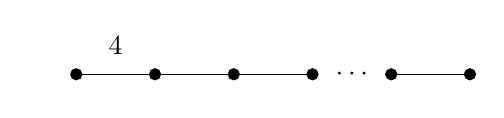
\begin{tikzpicture}[scale=1.0]%B_{n}
\draw [fill=black] \foreach \x in {1,2,...,6} {(\x,8.5) circle (2pt)};
\draw {(.5,8.5) node{}
(1.5,8.5) node[label=above:$4$]{}
(4.5,8.5) node{$\cdots$}
[-] (1,8.5) -- (4,8.5)
[-] (5,8.5) -- (6,8.5)
(2,8.5) node{}}; 
\end{tikzpicture}
\caption{$B_{n}$} \label{fig:B}
\end{subfigure} \\

    & \\ 

\begin{subfigure}{0.5\textwidth} \centering
\begin{tikzpicture}[scale=1.0]
\draw[fill=black] \foreach \x in {1,2} {(\x,0) circle (2pt)};
\fill[fill=white] (2,1) circle (2pt);
\draw {(.25,0) node{}
(1.5,0) node[label=above:$m$]{}
[-] (1,0) -- (2,0)
(2,0) node{}};
\end{tikzpicture}
\caption{$I_{2}(m)$} \label{fig:I}
\end{subfigure} &

\begin{subfigure}{0.5\textwidth} \centering
\begin{tikzpicture}[scale=1.0]
\draw[fill=black] \foreach \x in {1,2,...,6} {(\x,6.5) circle (2pt)};%D_{n}
\draw[fill=black] (2,7.5) circle (2pt);
\draw {(.5,6.5) node{}
(4.5,6.5) node{$\cdots$}
[-] (1,6.5) -- (4,6.5)
[-] (5,6.5) -- (6,6.5)
[-] (2,6.5) -- (2,7.5)
(2,6.5) node{}};
\end{tikzpicture}
\caption{$D_{n}$} \label{fig:D}
\end{subfigure} \\

    & \\ 
    
\begin{subfigure}{0.5\textwidth} \centering
\begin{tikzpicture}[scale=1.0]%E_{6}
\draw[fill=black] \foreach \x in {1,2,...,5} {(\x,4.5) circle (2pt)};
\draw[fill=black] (3,5.5) circle (2pt);
\draw {
[-] (1,4.5) -- (5,4.5)
[-] (3,4.5) -- (3,5.5)
(3,4.5) node{}};
\end{tikzpicture}
\caption{$E_{6}$} \label{fig:E6}
\end{subfigure} &



\begin{subfigure}{0.5\textwidth} \centering
\begin{tikzpicture}[scale=1.0]%E_{7}
\draw[fill=black] \foreach \x in {1,2,...,6} {(\x,4.5) circle (2pt)};
\draw[fill=black] (3, 5.5) circle (2pt);
\draw {
[-] (1,4.5) -- (5,4.5)
[-] (5,4.5) -- (6,4.5)
[-] (3,4.5) -- (3,5.5)
(3,4.5) node{}};
\end{tikzpicture}
\caption{$E_{7}$} \label{fig:E7}
\end{subfigure} \\

    & \\ 


\begin{subfigure}{0.5\textwidth} \centering
\begin{tikzpicture}[scale=1.0]%E_{8}
\draw[fill=black] \foreach \x in {1,2,...,7} {(\x,4.5) circle (2pt)};
\draw[fill=black] (3,5.5) circle (2pt);
\draw {
[-] (1,4.5) -- (7,4.5)
[-] (3,4.5) -- (3,5.5)
(3,4.5) node{}};
\end{tikzpicture}
\caption{$E_{8}$} \label{fig:E6}
\end{subfigure} &

\begin{subfigure}{0.5\textwidth} \centering
\begin{tikzpicture}[scale=1.0]%F_{4}
\draw[fill=black] \foreach \x in {1,2,...,4} {(\x,3) circle (2pt)};
\fill[white] (1,4) circle (2pt);
\draw {(.5,3) node{}
(2.5,3) node[label=above:$4$]{}
[-] (1,3) -- (4,3)
(3,3) node{}};
\end{tikzpicture}
\caption{$F_{4}$} \label{fig:F4}
\end{subfigure} \\

&\\

\begin{subfigure}{0.5\textwidth} \centering
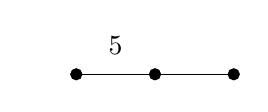
\begin{tikzpicture}[scale=1.0]
\draw[fill=black] \foreach \x in {1,2,...,3} {(\x,1.5) circle (2pt)};%H_{3}
\draw {(.5,1.5) node{}
(1.5,1.5) node[label=above:$5$]{}
[-] (1,1.5) -- (3,1.5)
(2,1.5) node{}}; 
\end{tikzpicture}
\caption{$H_{3}$} \label{fig:H}
\end{subfigure} &

\begin{subfigure}{0.5\textwidth} \centering
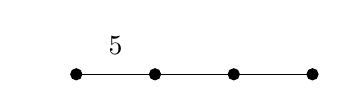
\begin{tikzpicture}[scale=1.0]
\draw[fill=black] \foreach \x in {1,2,...,4} {(\x,1.5) circle (2pt)};%H_{4}
\draw {(.5,1.5) node{}
(1.5,1.5) node[label=above:$5$]{}
[-] (1,1.5) -- (4,1.5)
(2,1.5) node{}}; 
\end{tikzpicture}
\caption{$H_{4}$} \label{fig:H}
\end{subfigure}
\end{tabular}
\caption{Coxeter graphs corresponding to the irreducible finite Coxeter sytems.}
\label{fig:fincoxgraphs}
\end{figure}

%%%%%%%%%%%%%%%%%%%%%%%%%%%

\begin{figure}[h!]
\begin{tabular}{m{7cm} m{7cm}}
\begin{subfigure}{0.5\textwidth} \centering
\begin{tikzpicture}[scale=1.0]%\widetilde{A}_{2}
\draw[fill=black] \foreach \x in {1,2} {(\x,10) circle (2pt)};
\fill[white] (1,11) circle (2pt);
\draw { (.5,10) node{}
(1.5,10) node[label=above:$\infty$]{}
[-] (1,10) -- (2,10)
(1,10) node{}}; 
\end{tikzpicture}
\caption{$\widetilde{A}_{2}$} \label{fig:affA2}
\end{subfigure} &

\begin{subfigure}{0.5\textwidth} \centering
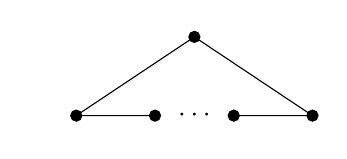
\begin{tikzpicture}[scale=1.0]%\widetilde{A}_{n}
\draw [fill=black] \foreach \x in {1,...,4} {(\x,7.5) circle (2pt)};
\draw [fill=black] (2.5, 8.5) circle (2pt);
\draw {(.5,8.5) node{}
(2.5,7.5) node{$\cdots$}
[-] (2.5,8.5) -- (1, 7.5)
[-] (2.5,8.5) -- (4, 7.5)
[-] (1,7.5) -- (2,7.5)
[-] (3,7.5) -- (4,7.5)
(2,8.5) node{}}; 
\end{tikzpicture}
\caption{$\widetilde{A}_{n}$} \label{fig:affAn}
\end{subfigure} \\

    & \\ 

\begin{subfigure}{0.5\textwidth} \centering
\begin{tikzpicture}[scale=1.0]%\widetilde{B}_{n}
\draw[fill=black] \foreach \x in {1,2,...,6} {(\x,0) circle (2pt)};
\draw[fill=black] (2,1) circle (2pt);
\draw {(.25,0) node{}
(5.5,0) node[label=above:$4$]{}
(4.5, 0) node{$\cdots$}
[-] (1,0) -- (4,0)
[-] (5,0) -- (6,0)
[-] (2,1) -- (2,0)
(2,0) node{}};
\end{tikzpicture}
\caption{$\widetilde{B}_{n}$} \label{fig:affB}
\end{subfigure} &

\begin{subfigure}{0.5\textwidth} \centering
\begin{tikzpicture}[scale=1.0]
\draw[fill=black] \foreach \x in {1,2,...,6} {(\x,5) circle (2pt)};%\widetild{C}_{n}
\fill[white] (1,6) circle (2pt);
\draw {(.5,5) node{}
(4.5,5) node{$\cdots$}
(5.5,5) node[label=above:$4$]{}
(1.5,5) node[label=above:$4$]{}
[-] (1,5) -- (4,5)
[-] (5,5) -- (6,5)
(2,5) node{}};
\end{tikzpicture}
\caption{$\widetilde{C}_{n}$} \label{fig:affC}
\end{subfigure} \\

    & \\ 
    
\begin{subfigure}{0.5\textwidth} \centering
\begin{tikzpicture}[scale=1.0]%\widetilde{D}_{6}
\draw[fill=black] \foreach \x in {1,2,...,6} {(\x,3.5) circle (2pt)};
\draw[fill=black] (2,4.5) circle (2pt);
\fill[white] (2,5.5) circle (2pt);
\draw[fill=black] (5,4.5) circle (2pt);
\draw {
(3.5,3.5) node{$\cdots$}
[-] (1,3.5) -- (3,3.5)
[-] (4, 3.5) --(6, 3.5)
[-] (2,3.5) -- (2,4.5)
[-] (5,3.5)-- (5,4.5)
(3,4.5) node{}};
\end{tikzpicture}
\caption{$\widetilde{D}_{n}$} \label{fig:E6}
\end{subfigure} &



\begin{subfigure}{0.5\textwidth} \centering
\begin{tikzpicture}[scale=1.0]%\widetilde{E}_{6}
\draw[fill=black] \foreach \x in {1,2,...,5} {(\x,4.5) circle (2pt)};
\draw[fill=black] (3, 5.5) circle (2pt);
\draw[fill=black] (3, 6.5) circle (2pt);
\draw {
[-] (1,4.5) -- (5,4.5)
[-] (3,4.5) -- (3,6.5)
(3,4.5) node{}};
\end{tikzpicture}
\caption{$\widetilde{E}_{6}$} \label{fig:affE6}
\end{subfigure} \\

    & \\ 


\begin{subfigure}{0.5\textwidth} \centering
\begin{tikzpicture}[scale=1.0]%\widetilde{E}_{7}
\draw[fill=black] \foreach \x in {1,2,...,7} {(\x,4.5) circle (2pt)};
\draw[fill=black] (4,5.5) circle (2pt);
\draw {
[-] (1,4.5) -- (7,4.5)
[-] (4,4.5) -- (4,5.5)
(3,4.5) node{}};
\end{tikzpicture}
\caption{$\widetilde{E}_{7}$} \label{fig:affE7}
\end{subfigure} &

\begin{subfigure}{0.5\textwidth} \centering
\begin{tikzpicture}[scale=1.0]%\widetilde{E}_{8}
\draw[fill=black] \foreach \x in {1,2,...,8} {(\x,3) circle (2pt)};
\draw[fill=black] (3,4) circle (2pt);
\draw {(.5,3) node{}
[-] (3,4) -- (3,3)
[-] (1,3) -- (8,3)
(3,3) node{}};
\end{tikzpicture}
\caption{$\widetilde{E}_{8}$} \label{fig:affE8}
\end{subfigure} \\

&\\

\begin{subfigure}{0.5\textwidth} \centering
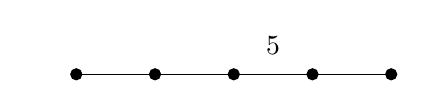
\begin{tikzpicture}[scale=1.0]
\draw[fill=black] \foreach \x in {1,2,...,5} {(\x,1.5) circle (2pt)};%\widetilde{F}_{4}
\draw {(.5,1.5) node{}
(3.5,1.5) node[label=above:$5$]{}
[-] (1,1.5) -- (5,1.5)
(2,1.5) node{}}; 
\end{tikzpicture}
\caption{$\widetilde{F}_{4}$} \label{fig:H}
\end{subfigure} &

\begin{subfigure}{0.5\textwidth} \centering
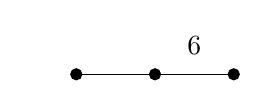
\begin{tikzpicture}[scale=1.0]
\draw[fill=black] \foreach \x in {1,2,...,3} {(\x,1.5) circle (2pt)};%\widetilde{G}_{2}
\draw {(.5,1.5) node{}
(2.5,1.5) node[label=above:$6$]{}
[-] (1,1.5) -- (3,1.5)
(2,1.5) node{}}; 
\end{tikzpicture}
\caption{$\widetilde{G}_{4}$} \label{fig:H}
\end{subfigure}
\end{tabular}
\caption{Coxeter graphs corresponding to the irreducible affine Coxeter systems.}
\label{fig:infincoxgraphs}
\end{figure}

%%%%%%%%%%%%%%%%%%%%%%%%%%%


\section{Fully Commutative Elements}\label{sec:FC}
Let $(W,S)$ be a Coxeter system of type $\Gamma$ and let $w \in W$. Following~\cite{Stembridge1996}, we define a relation $\sim$ on the set of reduced expressions for $w$. Let $\overline{w}_1$ and $\overline{w}_2$ be two reduced expressions for $w$. We define $\overline{w}_1 \sim \overline{w}_2$ if we can obtain $\overline{w}_2$ from $\overline{w}_1$ by applying a single commutation move of the form $st \mapsto ts$ where $m(s,t)=2$. Now, define the equivalence relation $\approx$ by taking the reflexive transitive closure of $\sim$. Each equivalence class under $\approx$ is called a \emph{commutation class}. If $w$ has a single commutation class, then we say that $w$ is \emph{fully commutative} (FC). 

The set of FC elements of $W(\Gamma)$ is denoted by $\FC(\Gamma)$. Given some $w \in \FC(\Gamma)$, and a starting reduced expression for $w$, observe the definition of FC states that one only needs to perform commutations to obtain all reduced expressions for $w$, but the following result due to Stembridge~\cite{Stembridge1996} states that when $w$ is FC performing commutations is the only possible way to obtain another reduced expression for $w$.

\begin{theorem}[Stembridge,~\cite{Stembridge1996}]\label{thm:Stembridge}
	Let $(W,S)$ be a Coxeter system. An element $w \in W$ is FC if and only if no reduced expression for $w$ contains $\underbrace{sts\cdots}_{m(s,t)}$ as a subword for all when $m(s,t) \geq 3$. \qed
\end{theorem}

In other words, $w$ is FC if and only if we never have the opportunity to apply a braid move.

\begin{example}
	Let $w \in W(\widetilde{C}_4)$ and let $\overline{w}=s_0s_1s_2s_0s_3s_1$ be a reduced expression for $w$. We see that
	\[s_0s_1\textcolor{purple}{s_2s_0}s_3s_1=s_0s_1s_0s_2\textcolor{purple}{s_3s_1}=s_0s_1s_0s_2s_1s_3,\]
	where the \textcolor{purple}{purple} indicates applying a commutation. Note that there is no possible way to perform a braid move. Hence $w$ is $\FC$.
\end{example}

\begin{example}
Let $\overline{w}=s_1s_0s_4s_1s_3s_5s_2s_4s_6$ be a reduced expression for $w \in \FC(\widetilde{C}_6)$. Applying the commutation $s_4s_2=s_2s_4$, we can obtain another reduced expression for $w$, namely $\overline{w}_2=s_1s_0s_4s_1s_3s_5s_4s_2s_6$ which is in the same commutation class as $\overline{w_1}$. However, applying the braid move $s_2s_3s_2=s_3s_2s_3$, we obtain another reduced expression $\overline{w_3}=s_1s_3s_2s_3s_4s_0$. Note that since $\overline{w}_3$ was obtained by applying a braid move, $\overline{w_3}$ is in a different commutation class than $\overline{w_1}$ and $\overline{w_2}$. It turns out $w$ has exactly two commutation classes, one containing $\overline{w}_1$ and $\overline{w}_2$ and another containing $\overline{w}_3$. So $w$ is not FC.
\end{example}

\begin{example}
Let $w \in W(\widetilde{C}_4)$ and let $\overline{w}=s_0s_1s_2s_0s_1s_2$ be a reduced expression for $w$. We see that
\[s_0s_1\textcolor{purple}{s_3s_0}s_1s_2=s_0s_1s_0\textcolor{purple}{s_3s_1}s_2=\textcolor{orange}{s_0s_1s_0s_1}s_3s_2,\]
where the \textcolor{purple}{purple} indicates applying a commutation and the \textcolor{orange}{orange} indicates applying a braid move. Thus $w$ is not $\FC$ by Theorem~\ref{thm:Stembridge}.  	
\end{example}

Stembridge classified the irreducible Coxeter Systems that contain a finite number of FC elements, the so-called \emph{FC-finite Coxeter groups}. This thesis is mainly concerned with $W(A_n),~W(B_n),\text{ and }W(\widetilde{C}_n)$. Both $W(A_n)~\mathrm{and}~W(B_n)$ are finite Coxeter groups, and thus are $\FC$-finite. On the other hand, $W(\widetilde{C}_n)$ is infinite and has infinitely many $\FC$ elements. However, there exist some infinite Coxeter groups that contain finitely many $\FC$ elements. For example, $E_n$ for $n \geq 9$ (see Figure~\ref{fig:FCfincoxgraphs}) is infinite, but contains only finitely many FC elements.

\begin{theorem}[Stembridge,~\cite{Stembridge1996}]
\label{thm:FCfinite} The FC-finite irreducible Coxeter systems are of type $A_n$ with $n \geq 1$, $B_n$ with $n \geq 2$, $D_n$ with $n \geq 4$, $E_n$ with $n \geq 6$, $F_n$ with $n \geq 4$, $H_n$ with $n \geq 3$, and $I_2(m)$ with $5 \leq m < \infty$. \qed
\end{theorem} 
 
The irreducible FC-finite Coxeter graphs are given in Figure~\ref{fig:FCfincoxgraphs}. Note that we have already encountered some of the FC-finite Coxeter groups in Figure~\ref{fig:fincoxgraphs}. Since these are finite Coxeter groups it is clear that they will have a finite number of FC elements. However, we haven't yet encountered the Coxeter groups determined by graphs in Figures~\ref{fig:FCEn},~\ref{fig:FCFn},~\ref{fig:FCHn}. All of these Coxeter systems are infinite for large $n$, yet contain only finitely many FC elements.

\begin{figure}[h!]
\begin{tabular}{m{7cm} m{7cm}}
\begin{subfigure}{0.5\textwidth} \centering
\begin{tikzpicture}[scale=1.0]%A_{n}
\draw[fill=black] \foreach \x in {1,2,...,6} {(\x,10) circle (2pt)};
\draw {(.5,10) node{}
(1.5,10) node[label=above:\textcolor{white}{$4$}]{}
(4.5,10) node{$\cdots$}
[-] (1,10) -- (4,10)
[-] (5,10) -- (6,10)
(1,10) node{}}; 
\end{tikzpicture}
\caption{$A_{n}$} \label{fig:FCA}
\end{subfigure} &

\begin{subfigure}{0.5\textwidth} \centering
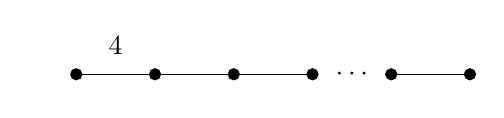
\begin{tikzpicture}[scale=1.0]%B_{n}
\draw [fill=black] \foreach \x in {1,2,...,6} {(\x,8.5) circle (2pt)};
\draw {(.5,8.5) node{}
(1.5,8.5) node[label=above:$4$]{}
(4.5,8.5) node{$\cdots$}
[-] (1,8.5) -- (4,8.5)
[-] (5,8.5) -- (6,8.5)
(2,8.5) node{}}; 
\end{tikzpicture}
\caption{$B_{n}$} \label{fig:FCB}
\end{subfigure} \\

    & \\ 

\begin{subfigure}{0.5\textwidth} \centering
\begin{tikzpicture}[scale=1.0]
\draw[fill=black] \foreach \x in {1,2,...,6} {(\x,6.5) circle (2pt)};%D_{n}
\draw[fill=black] (2,7.5) circle (2pt);
\draw {(.5,6.5) node{}
(4.5,6.5) node{$\cdots$}
[-] (1,6.5) -- (4,6.5)
[-] (5,6.5) -- (6,6.5)
[-] (2,6.5) -- (2,7.5)
(2,6.5) node{}};
\end{tikzpicture}
\caption{$D_{n}$} \label{fig:FCD}
\end{subfigure} &
    
\begin{subfigure}{0.5\textwidth} \centering
\begin{tikzpicture}[scale=1.0]%E_{6}
\draw[fill=black] \foreach \x in {1,2,...,6} {(\x,4.5) circle (2pt)};
\draw[fill=black] (3,5.5) circle (2pt);
%\fill[white] (3,5.9) circle (2pt);
\draw {(.5, 4.5) node{}
(4.5,4.5) node{$\cdots$}
[-] (1,4.5) -- (4,4.5)
[-] (5,4.5) -- (6,4.5)
[-] (3,4.5) -- (3,5.5)
(3,4.5) node{}};
\end{tikzpicture}
\caption{$E_{n}$} \label{fig:FCEn}
\end{subfigure} \\

&\\

\begin{subfigure}{0.5\textwidth} \centering
\begin{tikzpicture}[scale=1.0]%F_{n}
\draw[fill=black] \foreach \x in {1,2,...,6} {(\x,3) circle (2pt)};
\fill[white] (1,4) circle (2pt);
\draw {(.5,3) node{}
(2.5,3) node[label=above:$4$]{}
(4.5,3) node{$\cdots$}
[-] (1,3) -- (4,3)
[-] (5,3) -- (6,3)
(3,3) node{}};
\end{tikzpicture}
\caption{$F_{n}$} \label{fig:FCFn}
\end{subfigure} &


\begin{subfigure}{0.5\textwidth} \centering
\begin{tikzpicture}[scale=1.0]
\draw[fill=black] \foreach \x in {1,2,...,6} {(\x,1.5) circle (2pt)};%H_{4}
\fill[white] (1,2.5) circle (2pt);
\draw {(.5,1.5) node{}
(1.5,1.5) node[label=above:$5$]{}
(4.5,1.5) node{$\cdots$}
[-] (1,1.5) -- (4,1.5)
[-] (5,1.5) -- (6,1.5)
(2,1.5) node{}}; 
\end{tikzpicture}
\caption{$H_{n}$} \label{fig:FCHn}
\end{subfigure}
\end{tabular}
\caption{Coxeter graphs corresponding to the irreducible FC-finite Coxeter systems.}
\label{fig:FCfincoxgraphs}
\end{figure}
